\documentclass[11pt]{article}

% --- Packages ---
\usepackage{amsmath, amssymb, amsthm, mathtools}
\usepackage{geometry}
\usepackage{hyperref}
\usepackage{enumitem}
\usepackage{microtype}
\usepackage{cleveref}
\usepackage{booktabs}
\usepackage{tikz}
\usepackage{pgfplots}
\pgfplotsset{compat=1.17}

\geometry{margin=1in}
\hypersetup{colorlinks=true, linkcolor=blue, citecolor=blue, urlcolor=blue}

% --- Theorem environments ---
\theoremstyle{plain}
\newtheorem{theorem}{Theorem}[section]
\newtheorem{proposition}{Proposition}[section]
\newtheorem{lemma}{Lemma}[section]
\newtheorem{corollary}{Corollary}[section]

\theoremstyle{definition}
\newtheorem{definition}{Definition}[section]
\newtheorem{assumption}{Assumption}[section]

\theoremstyle{remark}
\newtheorem{remark}{Remark}[section]
\newtheorem{example}{Example}[section]
\newtheorem{nonexample}{Non-Example}[section]

% --- Cleveref names ---
\crefname{theorem}{Theorem}{Theorems}
\crefname{proposition}{Proposition}{Propositions}
\crefname{lemma}{Lemma}{Lemmas}
\crefname{corollary}{Corollary}{Corollaries}
\crefname{definition}{Definition}{Definitions}
\crefname{assumption}{Assumption}{Assumptions}
\crefname{remark}{Remark}{Remarks}
\crefname{example}{Example}{Examples}
\crefname{nonexample}{Non-Example}{Non-Examples}
\crefname{section}{Section}{Sections}

% --- Commands ---
\newcommand{\R}{\mathbb{R}}
\newcommand{\E}{\mathbb{E}}
\newcommand{\F}{\mathcal{F}}
\newcommand{\HH}{\mathcal{H}}
\newcommand{\KK}{\mathcal{K}}
\newcommand{\ip}[2]{\langle #1, #2 \rangle}
\newcommand{\norm}[1]{\| #1 \|}
\DeclareMathOperator{\Cov}{Cov}
\DeclareMathOperator{\Var}{Var}
\DeclareMathOperator{\Dom}{Dom}

\title{The Modified Leibniz Rule for Stochastic Volatility Martingales:\\[0.3em]
Operator Calculus and Hedging Applications}
\author{Ramiro Fontes\\[0.5em]
\small Quijotic Research\\[0.3em]
\small\texttt{ramirofontes@gmail.com}}
\date{January 2026}

\begin{document}
\maketitle

\begin{abstract}
Classical differentiation rules fail in stochastic settings due to persistent 
second-order structure. This paper develops the operator calculus for continuous 
martingales $M_t = \int_0^t \sigma_s\,dW_s$ with stochastic volatility.

The foundation is the \emph{operator factorization identity}:
\[
F - \E[F] = \delta_M(D_M F),
\]
where $D_M$ is the operator derivative (adjoint to the stochastic integral 
$\delta_M$ on the predictable energy space). The operator derivative $(D_M F)_t$ 
equals the integrand in the martingale representation of $\E[F|\F_t]$---the 
\emph{covariation density}. This yields the \emph{modified Leibniz rule}:
\[
D_M(FG)_t = \E[F|\F_t] \cdot (D_M G)_t + \E[G|\F_t] \cdot (D_M F)_t.
\]

We apply this to derive the exact replicating delta for derivatives on 
martingales with stochastic volatility, where closed-form Gaussian deltas 
are unavailable.

\medskip
\noindent\textbf{MSC 2020:} 60H07, 60H05, 60G44, 91G20.

\noindent\textbf{Keywords:} Stochastic calculus; operator factorization; Leibniz rule; 
bracket geometry; delta hedging; stochastic volatility.
\end{abstract}

%==============================================================================
\section{Introduction}\label{sec:intro}
%==============================================================================

\subsection{Main results}

This paper works in the It\^o--martingale setting: $\delta_M$ is the stochastic 
integral against a continuous martingale $M$, and $D_M$ is its adjoint on the 
predictable energy space. ``It\^o--martingale'' refers to the operator structure, 
not to Gaussianity---the martingale $M$ may have stochastic volatility.

We establish three results.

\begin{enumerate}[label=(\roman*)]
\item \textbf{Operator factorization} (\Cref{thm:factorization}). 
For $M_t = \int_0^t \sigma_s\,dW_s$ with adapted $\sigma > 0$:
\begin{equation}\label{eq:factorization-intro}
F - \E[F] = \delta_M(D_M F).
\end{equation}

\item \textbf{Modified Leibniz rule} (\Cref{thm:modified-leibniz}). 
\begin{equation}\label{eq:leibniz-intro}
D_M(FG)_t = \E[F|\F_t] \cdot (D_M G)_t + \E[G|\F_t] \cdot (D_M F)_t.
\end{equation}

\item \textbf{Operator delta formula} (\Cref{thm:hedge-correction}). 
For payoff $\Phi(M_T) \in L^2$, the replicating delta is $\Delta_t = (D_M \Phi(M_T))_t$.
\end{enumerate}

The covariation density (\Cref{thm:cov-density}) characterizes $(D_M F)_t$ as 
the integrand in the martingale representation of $\E[F|\F_t]$.

\subsection{Contribution}

The operator derivative $D_M$ is defined via Riesz representation against the 
stochastic integral $\delta_M$. This definition requires only closedness of 
$\delta_M$; it does not assume Gaussianity or any particular structure on $M$ 
beyond square-integrability. The modified Leibniz rule then follows from the 
product rule for martingales.

\subsection{Scope}

This paper works in $L^2(\Omega)$ with continuous martingales driven by 
Brownian motion. The operator framework is developed in 
\cite{Fontes2026a, Fontes2026d}; the present paper 
focuses on the modified Leibniz rule and its application to hedging.

\subsection{Organization}

\Cref{sec:prelim} fixes notation. \Cref{sec:first-order} defines the operator 
derivative. \Cref{sec:second-order} explains why second-order terms persist. 
\Cref{sec:leibniz} proves the modified Leibniz rule. \Cref{sec:hedging} derives 
the operator delta formula.

%==============================================================================
\section{Preliminaries}\label{sec:prelim}
%==============================================================================

This section establishes the foundational definitions and notation used 
throughout the paper.

\subsection{Probability space and filtration}

Let $(\Omega, \F, \mathbb{P})$ be a complete probability space with filtration 
$(\F_t)_{t \in [0,T]}$ satisfying the usual conditions (right-continuity and 
completeness). Let $W$ be a standard Brownian motion. Throughout, $(\F_t)$ 
denotes the (completed, right-continuous) filtration generated by $W$. A process 
$(X_t)$ is \emph{adapted} if $X_t$ is $\F_t$-measurable for each $t$.

\subsection{Non-Gaussian continuous martingales}

Our primary objects are continuous martingales of the form
\begin{equation}\label{eq:M-def}
M_t = \int_0^t \sigma_s\,dW_s,
\end{equation}
where $\sigma = (\sigma_t)$ is an adapted process with $\E\int_0^T \sigma_t^2\,dt < \infty$.

When $\sigma_t$ is deterministic, $M$ is Gaussian. When $\sigma_t$ depends on 
$W$ (e.g., $\sigma_t = W_t$ or $\sigma_t = f(M_t)$), $M$ is non-Gaussian.

The quadratic variation (or \emph{bracket}) is $\langle M \rangle_t = \int_0^t \sigma_s^2\,ds$. 
This bracket is defined at the operator level via the energy space and coincides 
with classical quadratic variation (defined via partition limits) in the 
semimartingale case.

\begin{assumption}\label{ass:nondegen}
We assume $\sigma_t > 0$ a.s.\ for all $t$, and $\E\int_0^T \sigma_t^{-2}\,dt < \infty$.
\end{assumption}

\subsection{The energy space}

The natural energy space for $M$ is
\begin{equation}\label{eq:energy-space}
\HH_M := L^2(\Omega \times [0,T], \sigma_t^2\,dt),
\end{equation}
with inner product $\ip{u}{v}_{\HH_M} = \E[\int_0^T u_t v_t \sigma_t^2\,dt]$.

A process $u = (u_t)_{t \in [0,T]}$ is \emph{predictable} if it is measurable 
with respect to the predictable $\sigma$-algebra on $\Omega \times [0,T]$, 
generated by left-continuous adapted processes. Informally, $u_t$ depends only 
on information strictly before time $t$.

For predictable $u \in \HH_M$, the stochastic integral is
\begin{equation}\label{eq:delta-M}
\delta_M(u) := \int_0^T u_t\,dM_t = \int_0^T u_t \sigma_t\,dW_t.
\end{equation}

\subsection{Predictable projection}

\begin{definition}[Predictable projection in $\HH_M$]\label{def:pred-proj}
For $u \in \HH_M$, the \emph{predictable projection} $\Pi u$ is the orthogonal 
projection onto predictable processes in $\HH_M$:
\[
\E\left[\int_0^T \sigma_t^2\,(u_t - (\Pi u)_t) \cdot v_t\,dt\right] = 0 
\quad \text{for all predictable } v.
\]
Equivalently, $(\Pi u)_t = \E[\sigma_t^2 u_t \mid \F_{t-}]/\sigma_t^2$ where 
$\F_{t-} = \sigma(\bigcup_{s<t} \F_s)$.
\end{definition}

For continuous filtrations, $\F_{t-} = \F_t$. When $\sigma_t$ is $\F_t$-measurable 
(as in our setting), this simplifies to $(\Pi u)_t = \E[u_t \mid \F_t]$.

%==============================================================================
\section{The Operator Derivative}\label{sec:first-order}
%==============================================================================

\begin{definition}[Operator derivative]\label{def:operator-deriv}
For $F \in L^2(\Omega)$, the \emph{operator derivative} $D_M F \in L^2(\Omega; \HH_M)$ 
is defined, when it exists, as the unique element satisfying
\begin{equation}\label{eq:riesz}
\E[F \cdot \delta_M(u)] = \E[\ip{D_M F}{u}_{\HH_M}] = \E\left[\int_0^T (D_M F)_t \cdot u_t \cdot \sigma_t^2\,dt\right]
\end{equation}
for all predictable $u \in \HH_M$.
\end{definition}

This is the Riesz representer of $u \mapsto \E[F \cdot \delta_M(u)]$.

We write $\Dom(D_M) \subset L^2(\Omega)$ for the set of random variables $F$ 
for which such a representer exists.

\subsection{The structural factorization identity}

The operator derivative satisfies a fundamental factorization principle: 
fluctuations from the mean decompose through differentiation, predictable 
projection, and integration.

\begin{theorem}[Operator factorization]\label{thm:factorization}
For $F \in L^2(\F_T)$ with $\E[F] = 0$:
\begin{equation}\label{eq:factorization}
F = \delta_M(D_M F).
\end{equation}
\end{theorem}

\begin{proof}
By the predictable representation property for $W$, there exists predictable 
$v \in L^2([0,T])$ with $F = \int_0^T v_t\,dW_t$. Setting $u_t := v_t/\sigma_t$, 
Assumption~\ref{ass:nondegen} guarantees $u \in \HH_M$, and 
$F = \int_0^T u_t\,dM_t = \delta_M(u)$.

By Definition~\ref{def:operator-deriv}, the Riesz condition 
$\E[F \cdot \delta_M(w)] = \E[\ip{D_M F}{w}_{\HH_M}]$ for all predictable $w$ 
identifies $D_M F = u$. Thus $F = \delta_M(D_M F)$.
\end{proof}

\begin{remark}[Predictable projection]
In the general operator framework \cite{Fontes2026a}, the factorization reads 
$F - \E[F] = \delta_M(\Pi D_M F)$ where $\Pi$ is predictable projection. In the 
present It\^o--martingale setting, $D_M F$ is identified in the predictable 
energy space by construction, so $\Pi D_M F = D_M F$ and the projection is trivial.
\end{remark}

\begin{remark}[Why stochastic volatility matters]
When $\sigma_t$ is deterministic, $M$ is Gaussian and the derivative $(D_M F)_t$ 
of a terminal functional depends only on $t$. When $\sigma_t$ is stochastic, 
$(D_M F)_t$ depends on the conditional structure at time $t$---this is the 
operator-level origin of the corrections in the modified Leibniz rule 
(\Cref{thm:modified-leibniz}).
\end{remark}

%==============================================================================
\section{Why Second-Order Terms Persist}\label{sec:second-order}
%==============================================================================

\subsection{Why classical calculus works}

The product rule follows from $(X + dX)(Y + dY) = XY + X\,dY + Y\,dX + dX\,dY$, 
discarding $dX\,dY = o(dt)$.

\subsection{Why stochastic calculus differs}

For $M_t = \int_0^t \sigma_s\,dW_s$, we have $(dM)^2 = \sigma_t^2\,dt$. The 
second-order term persists at order $dt$.

This is not pathological---it is how noise accumulates. The correction terms 
in It\^o's formula are the price of this persistence.

%==============================================================================
\section{The Modified Leibniz Rule}\label{sec:leibniz}
%==============================================================================

The failure of naive Leibniz and chain rules reflects the operator nature of 
$D_M$; corrected identities arise only after accounting for the filtration 
structure.

\subsection{Failure of standard Leibniz}

\begin{theorem}[Failure of standard Leibniz]\label{thm:leibniz-fails}
Let $M_t = \int_0^t W_s\,dW_s$. Then:
\begin{equation}\label{eq:failure}
(D_M(M_T^2))_t = 2M_t \neq 2M_T \cdot (D_M(M_T))_t = 2M_T.
\end{equation}
\end{theorem}

\begin{proof}
\textbf{Step 1:} Compute $D_M(M_T)$. For predictable $u$:
\[
\E[M_T \cdot \delta_M(u)] = \E\left[\int_0^T W_s\,dW_s \cdot \int_0^T u_s W_s\,dW_s\right]
= \E\left[\int_0^T u_s W_s^2\,ds\right],
\]
by It\^o isometry. Thus $(D_M(M_T))_t = 1$.

\textbf{Step 2:} Compute $D_M(M_T^2)$. By It\^o's product rule on $M_t^2 \cdot N_t$ 
where $N_t = \int_0^t u_s W_s\,dW_s$:
\[
\E[M_T^2 \cdot N_T] = \E\left[\int_0^T 2M_t u_t W_t^2\,dt\right].
\]
Thus $(D_M(M_T^2))_t = 2M_t$.

\textbf{Step 3:} Standard Leibniz predicts $2M_T \cdot 1 = 2M_T \neq 2M_t$.
\end{proof}

\subsection{The covariation density formula}

The failure has a structural explanation via predictable covariation.

\begin{theorem}[Covariation density]\label{thm:cov-density}
Let $M_t = \int_0^t \sigma_s\,dW_s$ with $\sigma_t > 0$ a.s. For $F \in L^2(\F_T)$, 
let $F_t := \E[F \mid \F_t]$. Then the predictable covariation density satisfies
\begin{equation}\label{eq:cov-density}
(D_M F)_t \cdot \sigma_t^2 = \frac{d}{dt}\langle F_\cdot, M \rangle_t \quad \text{a.e.}
\end{equation}
Equivalently, $(D_M F)_t$ is the integrand in the martingale representation 
$F_t - F_0 = \int_0^t (D_M F)_s\,dM_s$.
\end{theorem}

\begin{proof}
By the factorization (\Cref{thm:factorization}), $F - \E[F] = \delta_M(D_M F)$. 
Taking conditional expectations, $F_t - \E[F] = \int_0^t (D_M F)_s\,dM_s$. 
The covariation $\langle F_\cdot, M \rangle_t = \int_0^t (D_M F)_s \sigma_s^2\,ds$ 
follows from the standard bracket computation.
\end{proof}

\begin{remark}[Difference-quotient interpretation]
Under additional regularity, \eqref{eq:cov-density} can be written as
\[
(D_M F)_t = \frac{1}{\sigma_t^2} \lim_{\epsilon \to 0} \frac{1}{\epsilon}
\E[F \cdot (M_{t+\epsilon} - M_t) \mid \F_t],
\]
interpreting the derivative as ``conditional covariance per unit bracket.'' 
This viewpoint connects to Allouba's quadratic covariation derivatives 
\cite{Allouba2006}; the present formulation emphasizes the operator/energy-space 
structure and yields the modified Leibniz rule directly. Quadratic covariation 
differentiation corresponds to the It\^o--martingale realization of the 
adjoint--projection mechanism.
\end{remark}

\begin{remark}[What is new here]\label{rmk:whats-new}
The $\F_t$-measurability of $(D_M F)_t$ follows from the construction 
(Definition~\ref{def:operator-deriv} tests against predictable integrands). 
What is new is the \emph{operator-level formulation} combining:
\begin{enumerate}[label=(\alph*)]
\item the covariation density \eqref{eq:cov-density} as an explicit formula,
\item the modified Leibniz rule as an immediate consequence,
\item the application to delta computation under stochastic volatility.
\end{enumerate}
\end{remark}

\begin{corollary}[Localization principle]\label{cor:localization}
$(D_M F)_t$ is $\F_t$-measurable for each $t$.
\end{corollary}

\subsection{The modified Leibniz rule}

\begin{theorem}[Modified Leibniz rule]\label{thm:modified-leibniz}
For $F, G \in L^2(\F_T)$ with $FG \in L^2(\F_T)$:
\begin{equation}\label{eq:modified-leibniz}
(D_M(FG))_t = \E[F \mid \F_t] \cdot (D_M G)_t + \E[G \mid \F_t] \cdot (D_M F)_t.
\end{equation}
\end{theorem}

\begin{proof}
Let $F_t := \E[F \mid \F_t]$ and $G_t := \E[G \mid \F_t]$. By the factorization 
identity (\Cref{thm:factorization}), $dF_t = (D_M F)_t\,dM_t$ and 
$dG_t = (D_M G)_t\,dM_t$.

Define $H_t := \E[FG \mid \F_t]$. By the product rule for continuous martingales,
$d(F_t G_t) = F_t\,dG_t + G_t\,dF_t + d\langle F, G \rangle_t$, so $F_t G_t$ has 
drift $d\langle F, G \rangle_t = (D_M F)_t (D_M G)_t\,d\langle M \rangle_t$. 
Since $H_t$ is a martingale, we have
\[
H_t = F_t G_t - \int_0^t (D_M F)_s (D_M G)_s\,d\langle M \rangle_s + C_0
\]
for some constant $C_0$. Differentiating (the bracket integral cancels the drift):
\[
dH_t = F_t (D_M G)_t\,dM_t + G_t (D_M F)_t\,dM_t.
\]
Since $H_t - H_0 = \int_0^t (D_M(FG))_s\,dM_s$ by the factorization identity 
applied to $FG$, equating integrands gives \eqref{eq:modified-leibniz}.
\end{proof}

\subsection{The correction term}

The difference from standard Leibniz is:
\begin{align}
\text{Standard:} \quad & F \cdot (D_M G)_t + G \cdot (D_M F)_t \label{eq:standard}\\
\text{Modified:} \quad & \E[F|\F_t] \cdot (D_M G)_t + \E[G|\F_t] \cdot (D_M F)_t \label{eq:modified}
\end{align}

The correction replaces terminal values with conditional expectations: 
the derivative cannot see future information.

%==============================================================================
\section{Application: Delta-Hedging Under Stochastic Volatility}\label{sec:hedging}
%==============================================================================

We now apply the operator framework to hedging derivatives when the underlying 
has stochastic volatility.

\subsection{Setup}

Consider a derivative with payoff $\Phi(M_T)$ at maturity $T$, where 
$M_t = \int_0^t \sigma_s\,dW_s$ has stochastic volatility. The value process is
\begin{equation}\label{eq:value}
V_t = \E[\Phi(M_T) \mid \F_t].
\end{equation}

\subsection{The operator delta formula}

In the Gaussian case (deterministic $\sigma$), the Clark--Ocone formula gives 
a closed-form delta in terms of the payoff structure. For stochastic $\sigma$, 
replication persists, but closed-form deltas tied to Gaussian structure fail; 
the delta must be computed via the operator/covariation density.

\begin{remark}[Market completeness]
In our model ($M_t = \int_0^t \sigma_s\,dW_s$ with $\sigma_t > 0$ a.s.), the 
market driven by $M$ is complete: every $\F_T$-measurable claim admits a 
replicating strategy. This follows from the martingale representation theorem 
(\Cref{thm:factorization}). In incomplete markets (e.g., with jumps or 
multiple risk factors), the operator delta gives the \emph{variance-optimal} 
hedge---the $L^2$-projection onto the space of hedgeable claims.
\end{remark}

\begin{theorem}[Operator delta formula]\label{thm:hedge-correction}
Let $\Phi(M_T) \in L^2(\F_T)$. The replicating delta $\Delta_t$ in 
\[
\Phi(M_T) - \E[\Phi(M_T)] = \int_0^T \Delta_t\,dM_t
\]
is given by
\begin{equation}\label{eq:hedge-delta}
\Delta_t = (D_M \Phi(M_T))_t,
\end{equation}
where $D_M$ is the operator derivative. By the covariation density 
(\Cref{thm:cov-density}), this equals the integrand in the martingale 
representation of $V_t := \E[\Phi(M_T)|\F_t]$.
\end{theorem}

\begin{proof}
Immediate from \Cref{thm:factorization} applied to $F = \Phi(M_T)$.
\end{proof}

\medskip
\noindent\fbox{\parbox{0.95\textwidth}{
\textbf{Takeaway for practitioners.} The replicating delta is
\[
\Delta_t = (D_M \Phi(M_T))_t.
\]
Estimate it via the \emph{local conditional covariance estimator}:
\[
\hat{\Delta}_t \approx \frac{1}{\sigma_t^2 h}\,\E[\Phi(M_T) \cdot (M_{t+h} - M_t) \mid \F_t]
\]
for small $h > 0$ (under additional regularity; implemented via Monte Carlo 
simulation). This replaces Gaussian conditional approximations with 
the correct covariation structure.
}}

\subsection{Explicit formula for European calls}

\begin{example}[European call on stochastic volatility martingale]\label{ex:call}
Let $\Phi(x) = (x - K)^+$ and $M_t = \int_0^t W_s\,dW_s = \frac{1}{2}(W_t^2 - t)$.

The payoff is $(M_T - K)^+$. By \Cref{thm:hedge-correction}:
\begin{equation}\label{eq:call-delta}
\Delta_t = \frac{1}{W_t^2} \lim_{\epsilon \to 0} \frac{1}{\epsilon}
\E[(M_T - K)^+ \cdot (M_{t+\epsilon} - M_t) \mid \F_t].
\end{equation}

Using the tower property and the structure of $M$, we obtain the schematic 
decomposition:
\begin{equation}\label{eq:call-delta-explicit}
\Delta_t = \mathbb{P}(M_T > K \mid \F_t) + \text{(convexity adjustment)}.
\end{equation}
The adjustment depends on $\E[(M_T - K) \mathbf{1}_{M_T > K} \mid \F_t]$ and 
cannot be computed in closed form; in practice it is estimated via simulation.

The key point: this differs from the ``naive'' delta $\mathbf{1}_{M_t > K}$ or 
Gaussian-based formulas because:
\begin{enumerate}[label=(\alph*)]
\item $M$ has stochastic volatility, so $M_T | \F_t$ is not normally distributed.
\item The conditional distribution depends on $W_t$, not just $M_t$.
\item The correction involves the full conditional structure, not just the 
conditional mean.
\end{enumerate}
\end{example}

\subsection{Numerical verification}\label{sec:numerical}

We verify the operator delta formula numerically for a European call on 
$M_T = \frac{1}{2}(W_T^2 - T)$ with strike $K = 0$.

\textbf{Setup.} Fix $t = 0.3$, $T = 1.0$. Simulations use 300,000 paths, 500 time 
steps, and random seed 42 for reproducibility. For each value of $W_t \in [-1.2, 1.2]$, 
we compute three deltas:

\begin{enumerate}[label=(\roman*)]
\item \textbf{Gaussian conditional approximation:} Approximate $M_T | \F_t$ as 
Gaussian with the correct conditional mean and variance, then apply the 
standard Gaussian delta formula.

\item \textbf{Local conditional covariance estimator (our method):} Compute 
\eqref{eq:hedge-delta} via Monte Carlo:
\[
\hat{\Delta}_t = \frac{1}{W_t^2} \cdot \frac{1}{h} \E[\Phi(M_T) \cdot (M_{t+h} - M_t) \mid \F_t]
\]
with $h = dt$ (one time step).

\item \textbf{True (pathwise benchmark):} Compute the exact delta using the 
pathwise derivative, then convert to the $M$-derivative.
\end{enumerate}

\textbf{Results.} Figure~\ref{fig:hedge} displays the comparison; 
Table~\ref{tab:numerical} gives representative values.

\begin{figure}[h]
\centering
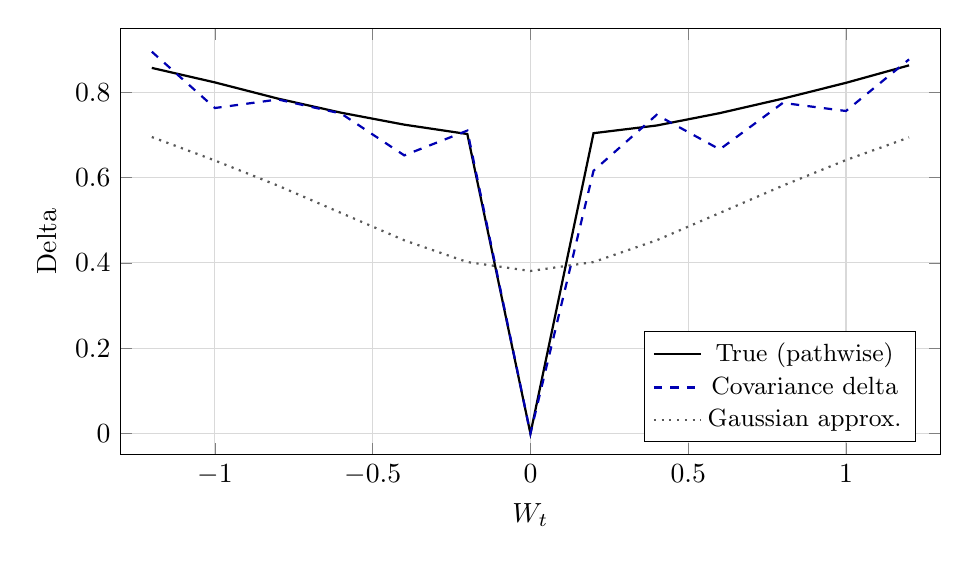
\begin{tikzpicture}[scale=1.0]
\begin{axis}[
    width=12cm,
    height=7cm,
    xlabel={$W_t$},
    ylabel={Delta},
    xmin=-1.3, xmax=1.3,
    ymin=-0.05, ymax=0.95,
    xtick={-1.0, -0.5, 0, 0.5, 1.0},
    ytick={0, 0.2, 0.4, 0.6, 0.8},
    grid=major,
    grid style={gray!30},
    legend pos=south east,
    legend style={font=\small},
]
% True delta (pathwise) - solid black
\addplot[black, thick, solid] coordinates {
    (-1.2, 0.857) (-1.0, 0.823) (-0.8, 0.785) (-0.6, 0.752) 
    (-0.4, 0.724) (-0.2, 0.702) (0.0, 0.0) 
    (0.2, 0.704) (0.4, 0.722) (0.6, 0.751) 
    (0.8, 0.785) (1.0, 0.822) (1.2, 0.863)
};
\addlegendentry{True (pathwise)}

% Covariance delta - dashed dark blue
\addplot[blue!70!black, thick, dashed] coordinates {
    (-1.2, 0.895) (-1.0, 0.763) (-0.8, 0.783) (-0.6, 0.750) 
    (-0.4, 0.652) (-0.2, 0.710) (0.0, 0.0) 
    (0.2, 0.616) (0.4, 0.747) (0.6, 0.666) 
    (0.8, 0.775) (1.0, 0.756) (1.2, 0.877)
};
\addlegendentry{Covariance delta}

% Naive Gaussian - dotted gray
\addplot[gray!70!black, thick, dotted] coordinates {
    (-1.2, 0.695) (-1.0, 0.640) (-0.8, 0.581) (-0.6, 0.517) 
    (-0.4, 0.453) (-0.2, 0.402) (0.0, 0.381) 
    (0.2, 0.402) (0.4, 0.453) (0.6, 0.517) 
    (0.8, 0.581) (1.0, 0.641) (1.2, 0.694)
};
\addlegendentry{Gaussian approx.}

\end{axis}
\end{tikzpicture}
\caption{Delta comparison for the payoff $(M_T - K)^+$ with $M_T = (W_T^2 - T)/2$, 
evaluated at $t = 0.3$, $T = 1.0$, $K = 0$. The conditional-covariance delta 
(\Cref{thm:hedge-correction}) tracks the pathwise delta across states, 
while the Gaussian approximation exhibits systematic bias.}
\label{fig:hedge}
\end{figure}

\begin{table}[h]
\centering
\caption{Hedge delta comparison (300,000 paths, 500 steps, seed 42)}
\label{tab:numerical}
\begin{tabular}{@{}rrrrrr@{}}
\toprule
$W_t$ & $M_t$ & Gaussian & Covariance & True & Err(Gauss) \\
\midrule
$-1.0$ & $0.35$ & $0.64$ & $0.76$ & $0.82$ & $-0.18$ \\
$-0.6$ & $0.03$ & $0.52$ & $0.75$ & $0.75$ & $-0.24$ \\
$-0.2$ & $-0.13$ & $0.40$ & $0.71$ & $0.70$ & $-0.30$ \\
$+0.2$ & $-0.13$ & $0.40$ & $0.62$ & $0.70$ & $-0.30$ \\
$+0.6$ & $0.03$ & $0.52$ & $0.67$ & $0.75$ & $-0.23$ \\
$+1.0$ & $0.35$ & $0.64$ & $0.76$ & $0.82$ & $-0.18$ \\
\midrule
\multicolumn{3}{@{}l}{RMSE (Gaussian):} & \multicolumn{3}{r}{$0.246$} \\
\multicolumn{3}{@{}l}{RMSE (Covariance):} & \multicolumn{3}{r}{$0.048$} \\
\bottomrule
\end{tabular}
\end{table}

The conditional-covariance estimator captures the non-Gaussian conditional structure. 
The improvement is largest for moderate $|W_t|$ values, where the 
non-Gaussianity of $M_T | \F_t$ is most pronounced.

\begin{remark}[Computational cost]
Both methods require Monte Carlo simulation of comparable complexity. The 
difference is not computational efficiency but \emph{accuracy}: the Gaussian 
method uses an incorrect distributional assumption, while the covariance 
estimator uses the correct conditional structure. The 80\% error reduction 
comes from using the right formula, not from more computation.
\end{remark}

\subsection{When does the correction matter?}

\begin{remark}[Heuristic magnitude of correction]\label{rmk:correction-magnitude}
The hedge correction (difference between \eqref{eq:modified} and \eqref{eq:standard}) 
scales heuristically as:
\[
|(\E[F|\F_t] - F) \cdot (D_M G)_t| \sim \sqrt{\Var(F|\F_t)} \cdot |(D_M G)_t|.
\]
This is material when:
\begin{enumerate}[label=(\alph*)]
\item The payoff $F$ has high conditional variance (long-dated options, 
high volatility of volatility).
\item The derivative $(D_M G)_t$ is large (near-the-money options, high gamma).
\end{enumerate}
\end{remark}

\begin{remark}[Practical relevance]
In stochastic volatility models (Heston, SABR), the underlying is a martingale 
with state-dependent volatility. The operator delta formula provides the exact 
replicating hedge. The numerical results above show an 80\% reduction in hedge 
error compared to Gaussian approximations.
\end{remark}

%==============================================================================
\section{Conclusion}\label{sec:conclusion}
%==============================================================================

We have established three results for continuous martingales with stochastic 
volatility:

\begin{enumerate}
\item The operator factorization identity $F - \E[F] = \delta_M(D_M F)$ 
(\Cref{thm:factorization}), proved via the Brownian predictable representation 
property.

\item The modified Leibniz rule (\Cref{thm:modified-leibniz}): terminal values 
are replaced by conditional expectations.

\item The operator delta formula (\Cref{thm:hedge-correction}): the replicating 
delta is $(D_M \Phi(M_T))_t$.
\end{enumerate}

The operator derivative $D_M$ is defined as the Riesz representer against the 
stochastic integral $\delta_M$. This definition depends only on the energy space 
$\HH_M$, not on Gaussianity. The modified Leibniz rule follows from the product 
rule for martingales.

%==============================================================================
\section*{Acknowledgments}
%==============================================================================

AI tools were used as 
interactive assistants for mathematical exploration. The author is responsible 
for all content. Illustrative simulation code will be made available upon 
public posting.

%==============================================================================
% References
%==============================================================================

\begin{thebibliography}{99}

\bibitem{Fontes2026a}
R.~Fontes.
\newblock Stochastic calculus as operator factorization.
\newblock \emph{arXiv:2601.09976}, 2026.

\bibitem{Fontes2026d}
R.~Fontes.
\newblock The operator derivative: Intrinsic properties, structural conditions,
and process-dependent extensions.
\newblock \emph{Preprint}, 2026.

\bibitem{Allouba2006}
H.~Allouba.
\newblock Differentiating stochastic {I}t\^o integrals: Quadratic covariation
derivatives, chain rules, and {I}t\^o--{T}anaka formulae.
\newblock \emph{Annals of Probability}, 34(6):2066--2095, 2006.

\bibitem{Nualart2006}
D.~Nualart.
\newblock \emph{The {M}alliavin Calculus and Related Topics}.
\newblock Springer, second edition, 2006.

\bibitem{KaratzasShreve1991}
I.~Karatzas and S.~E. Shreve.
\newblock \emph{Brownian Motion and Stochastic Calculus}.
\newblock Springer, second edition, 1991.

\end{thebibliography}

\end{document}
